\textbf{Pre and post collision velocities}: By using the conservation of momentum and conservation of kinetic energy, we can derive the how pre and post collision velocities related. For binary elastic (?) collisions we can write (I think for inelastic collisions this is not valid, since we don't have KE conservation equation), 
\begin{align}
    v^\prime  &= \frac{1}{2} (v + v_* + |v-v_*| \omega) \\
    v_*^\prime  &= \frac{1}{2} (v + v_* - |v-v_*| \omega)
\end{align} where $\omega$ is a unit vector, $\omega \in S^2$. Note that, for binary elastic collisions, $|v-v_*| = |v^\prime-v_*^\prime|$.

In general $B : \R^3 \times \R^3 \times S^2 \rightarrow \R_{0}^+$ represents the probability of $v,v_*$ collide with a scattering direction $\omega$. The angle $\theta$, is the angle between the post collision relative vector and the pre-collision relative vector. Therefore, we can write, 
\begin{equation}
    cos\theta = \frac{\omega \cdot (v-v_*)}{|v-v_*|}
\end{equation}
There are several models for $B$, the collision kernel,
\begin{itemize}
    \item Maxwellian gas : $B(|v-v_*|,cos\theta) = const.$
    \item Hard sphere gas : $B(|v-v_*|,cos\theta) = const.|v-v_*|$
    \item Variable hard sphere (VHS) gas : $B(|v-v_*|,cos\theta) = const. |v-v_*|^\alpha$
\end{itemize}

%\newpage
%Constant cross-section $t_{end} = 10^{-6}$ s\\
%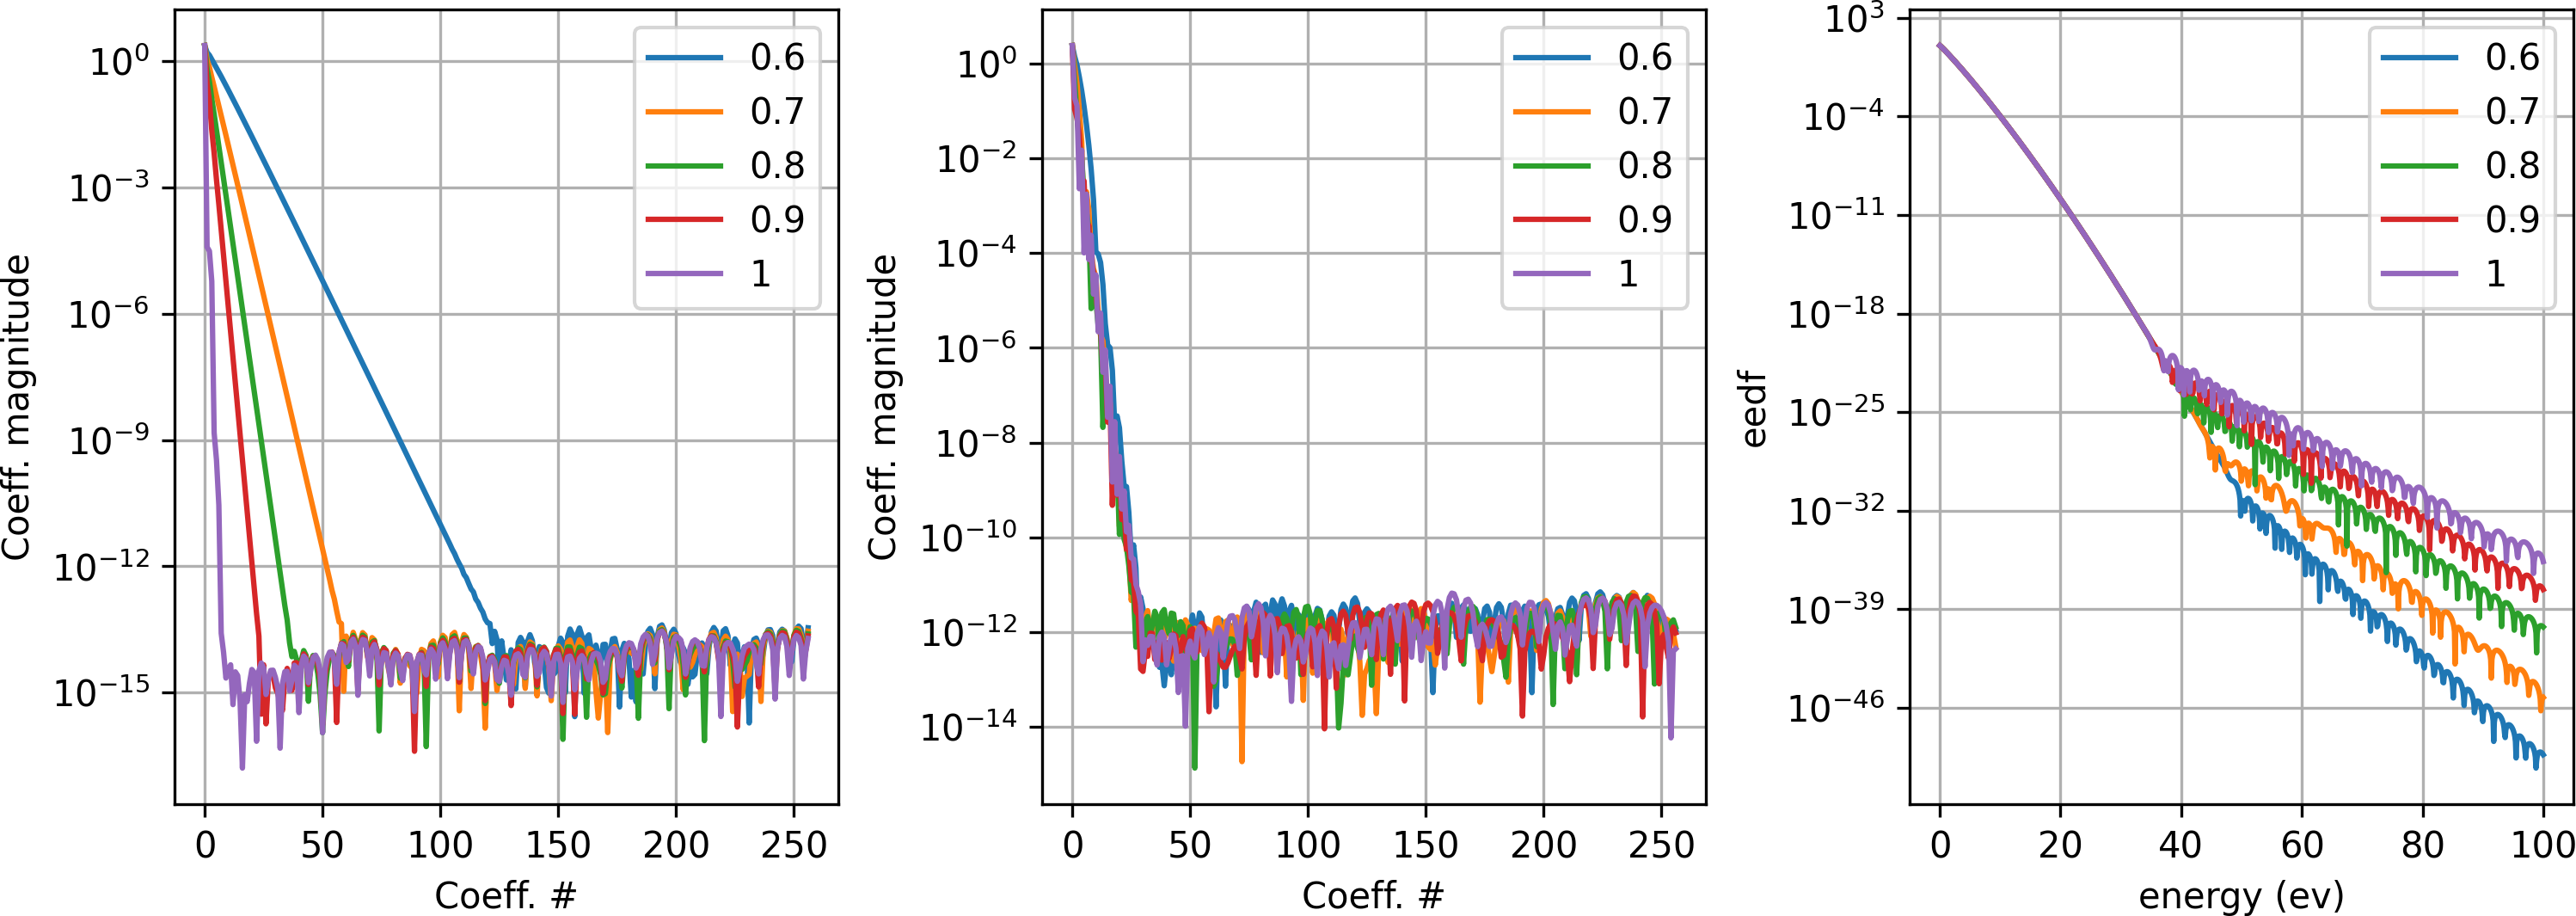
\includegraphics[width=0.99\textwidth]{fig/different_vth_const_1e-6.png}
%
%Data-fitted cross section $t_{end} = 10^{-6}$ s\\
%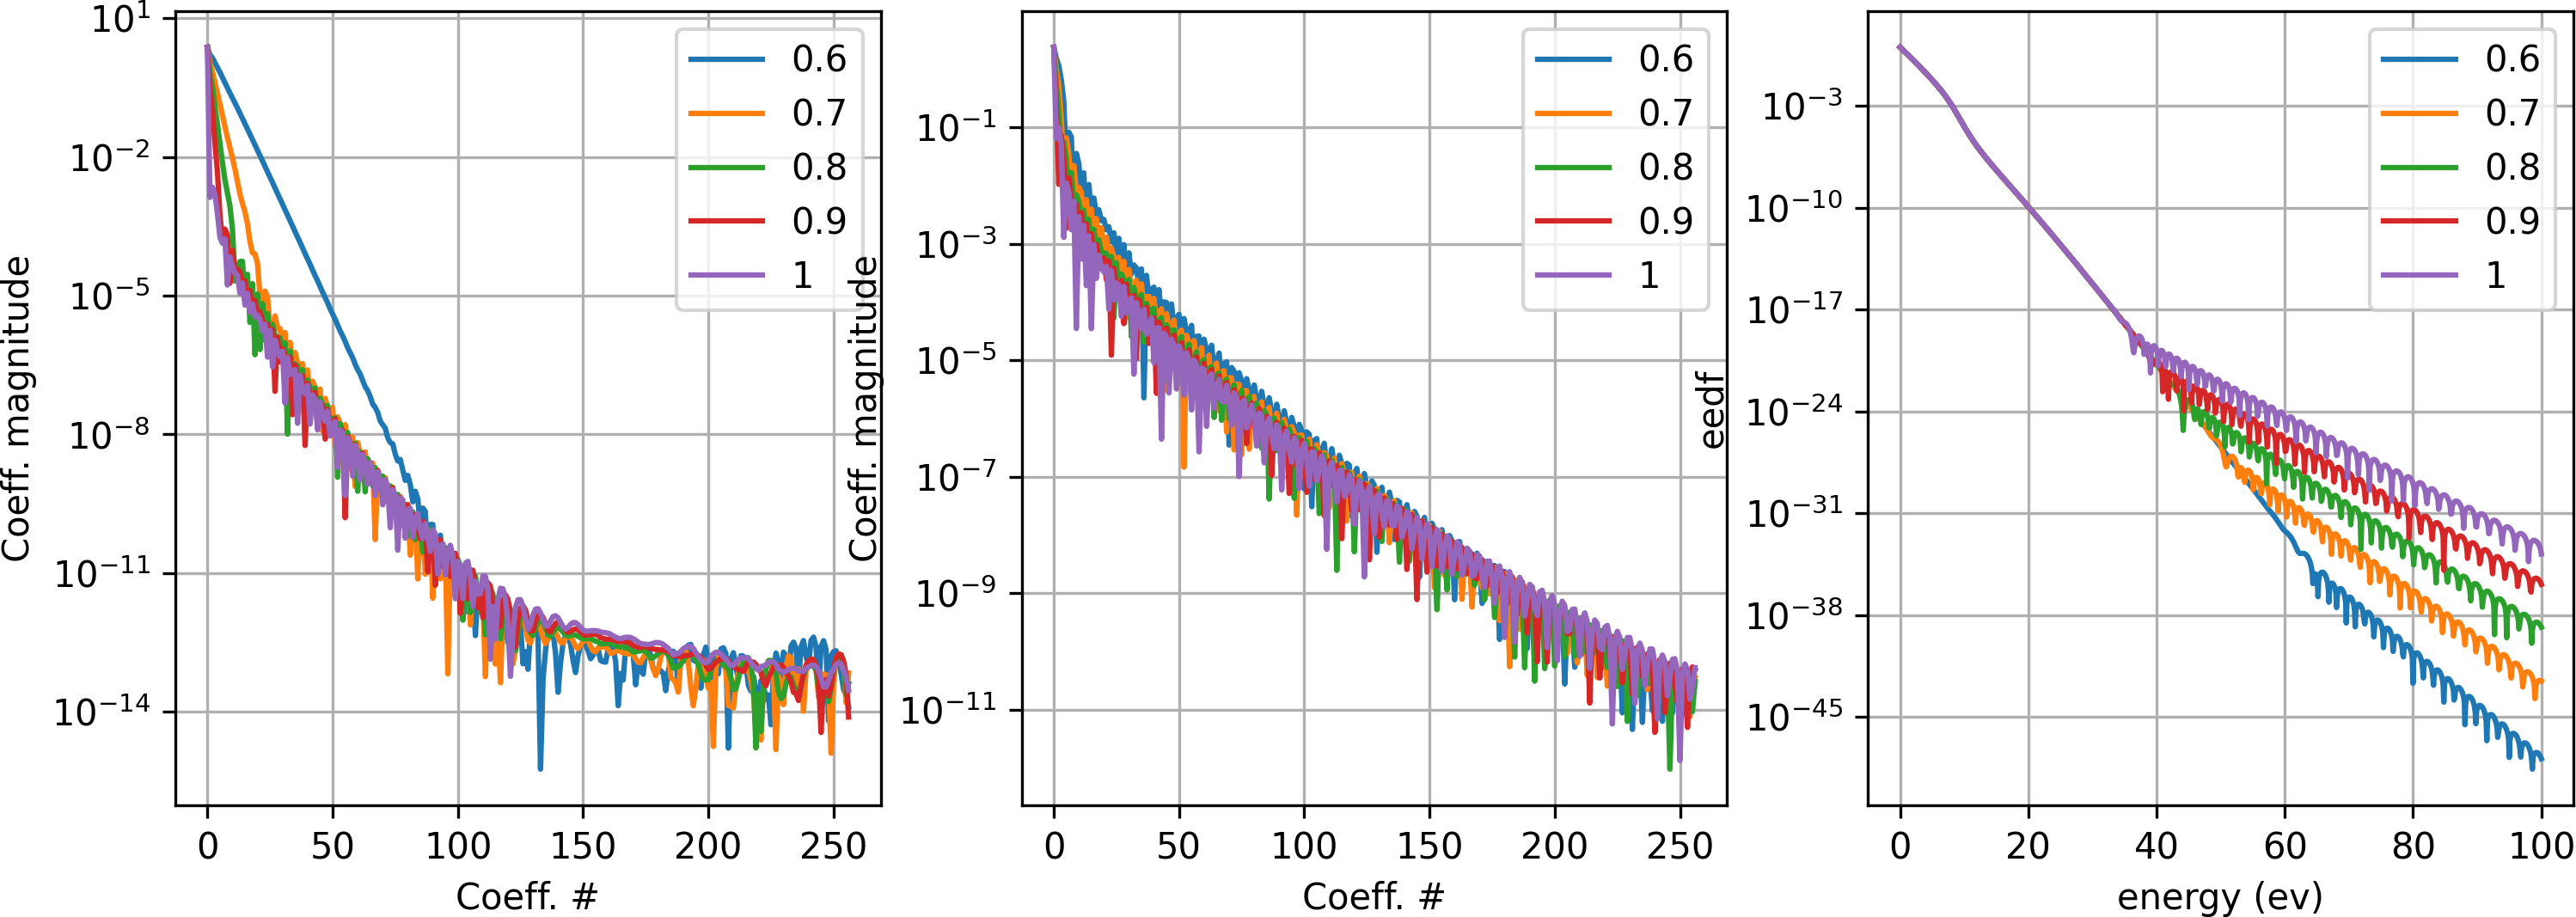
\includegraphics[width=0.99\textwidth]{fig/different_vth_real_1e-6.png}
%
%Constant cross-section $t_{end} = 10^{-5}$ s\\
%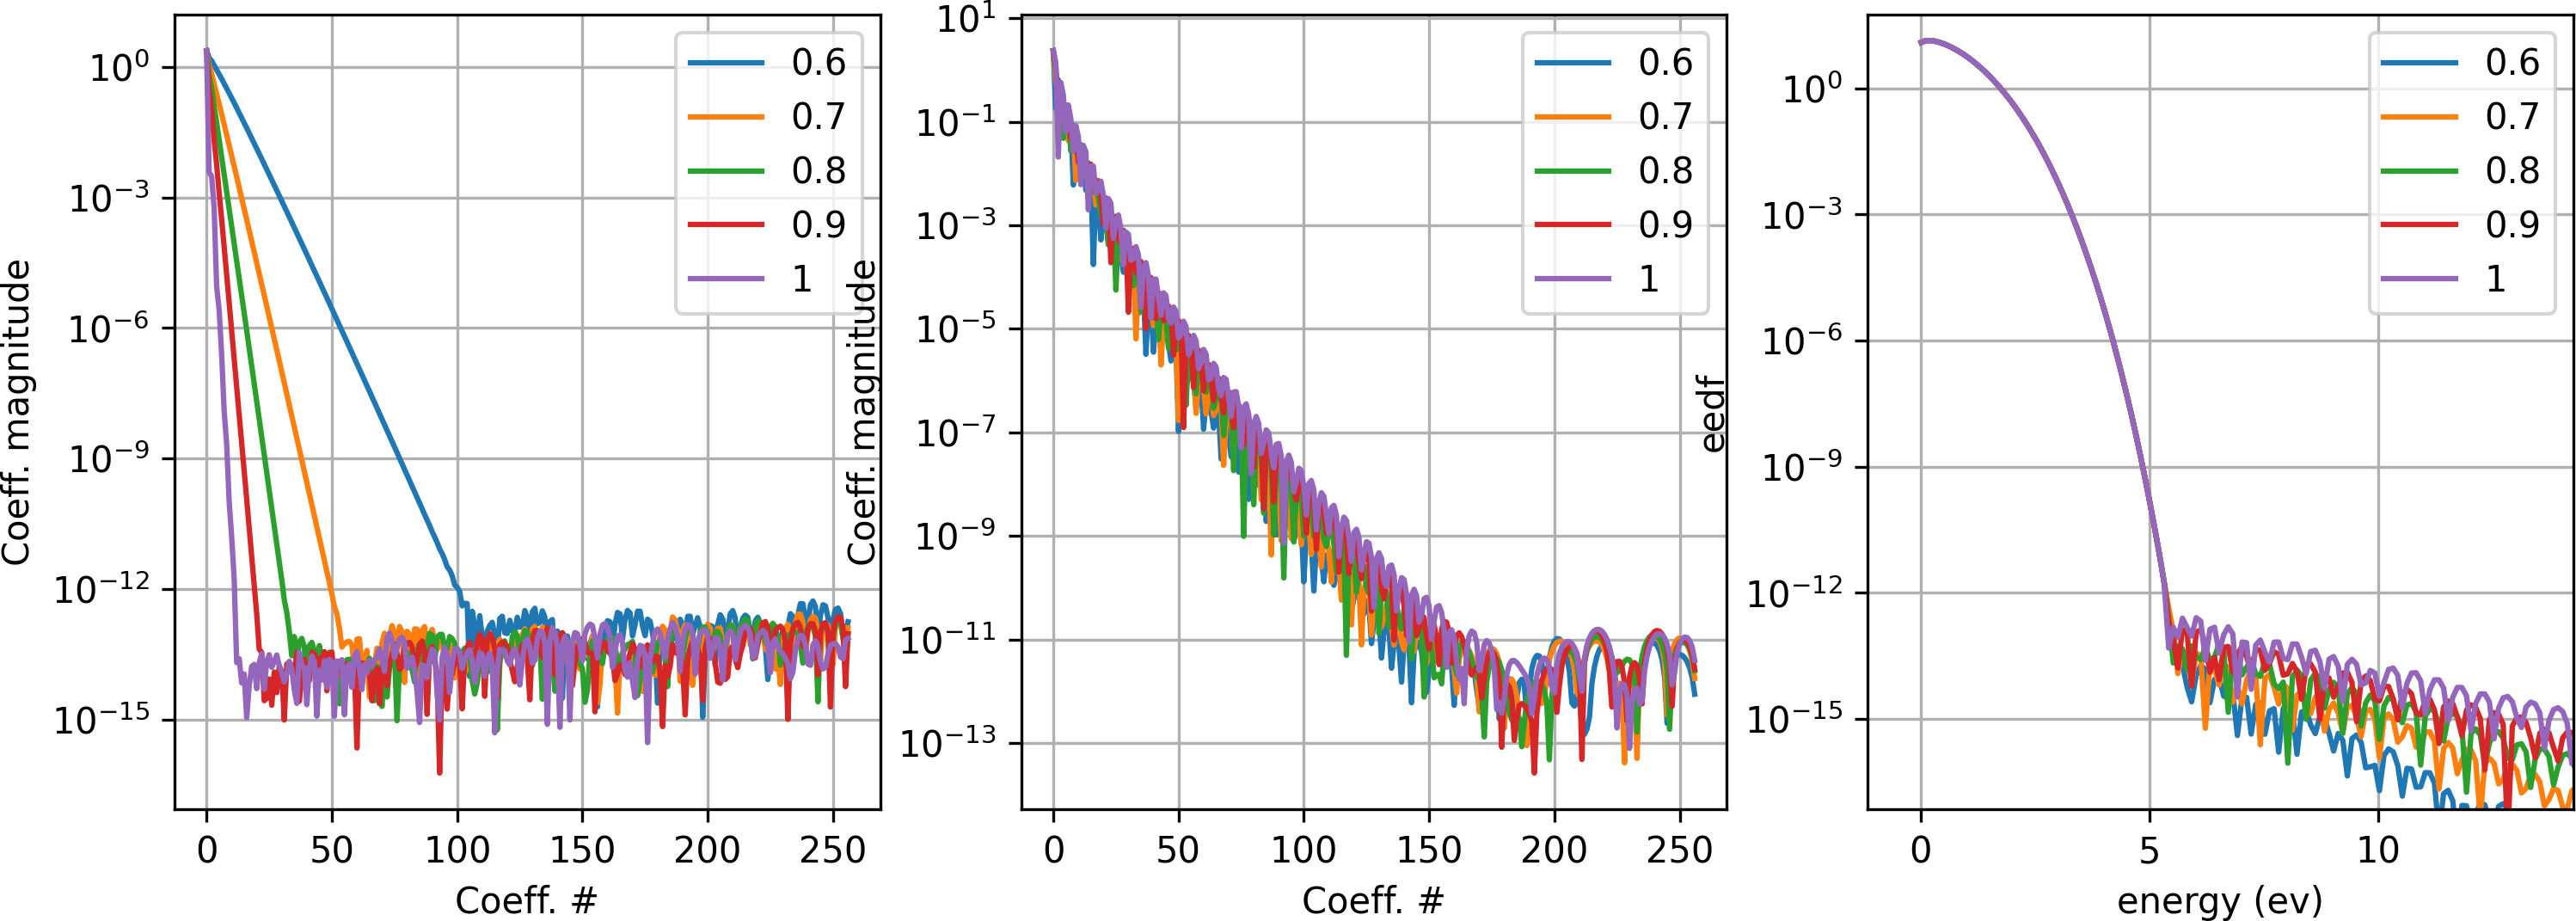
\includegraphics[width=0.99\textwidth]{fig/different_vth_const_1e-5.png}
%
%Data-fitted cross section $t_{end} = 10^{-5}$ s\\
%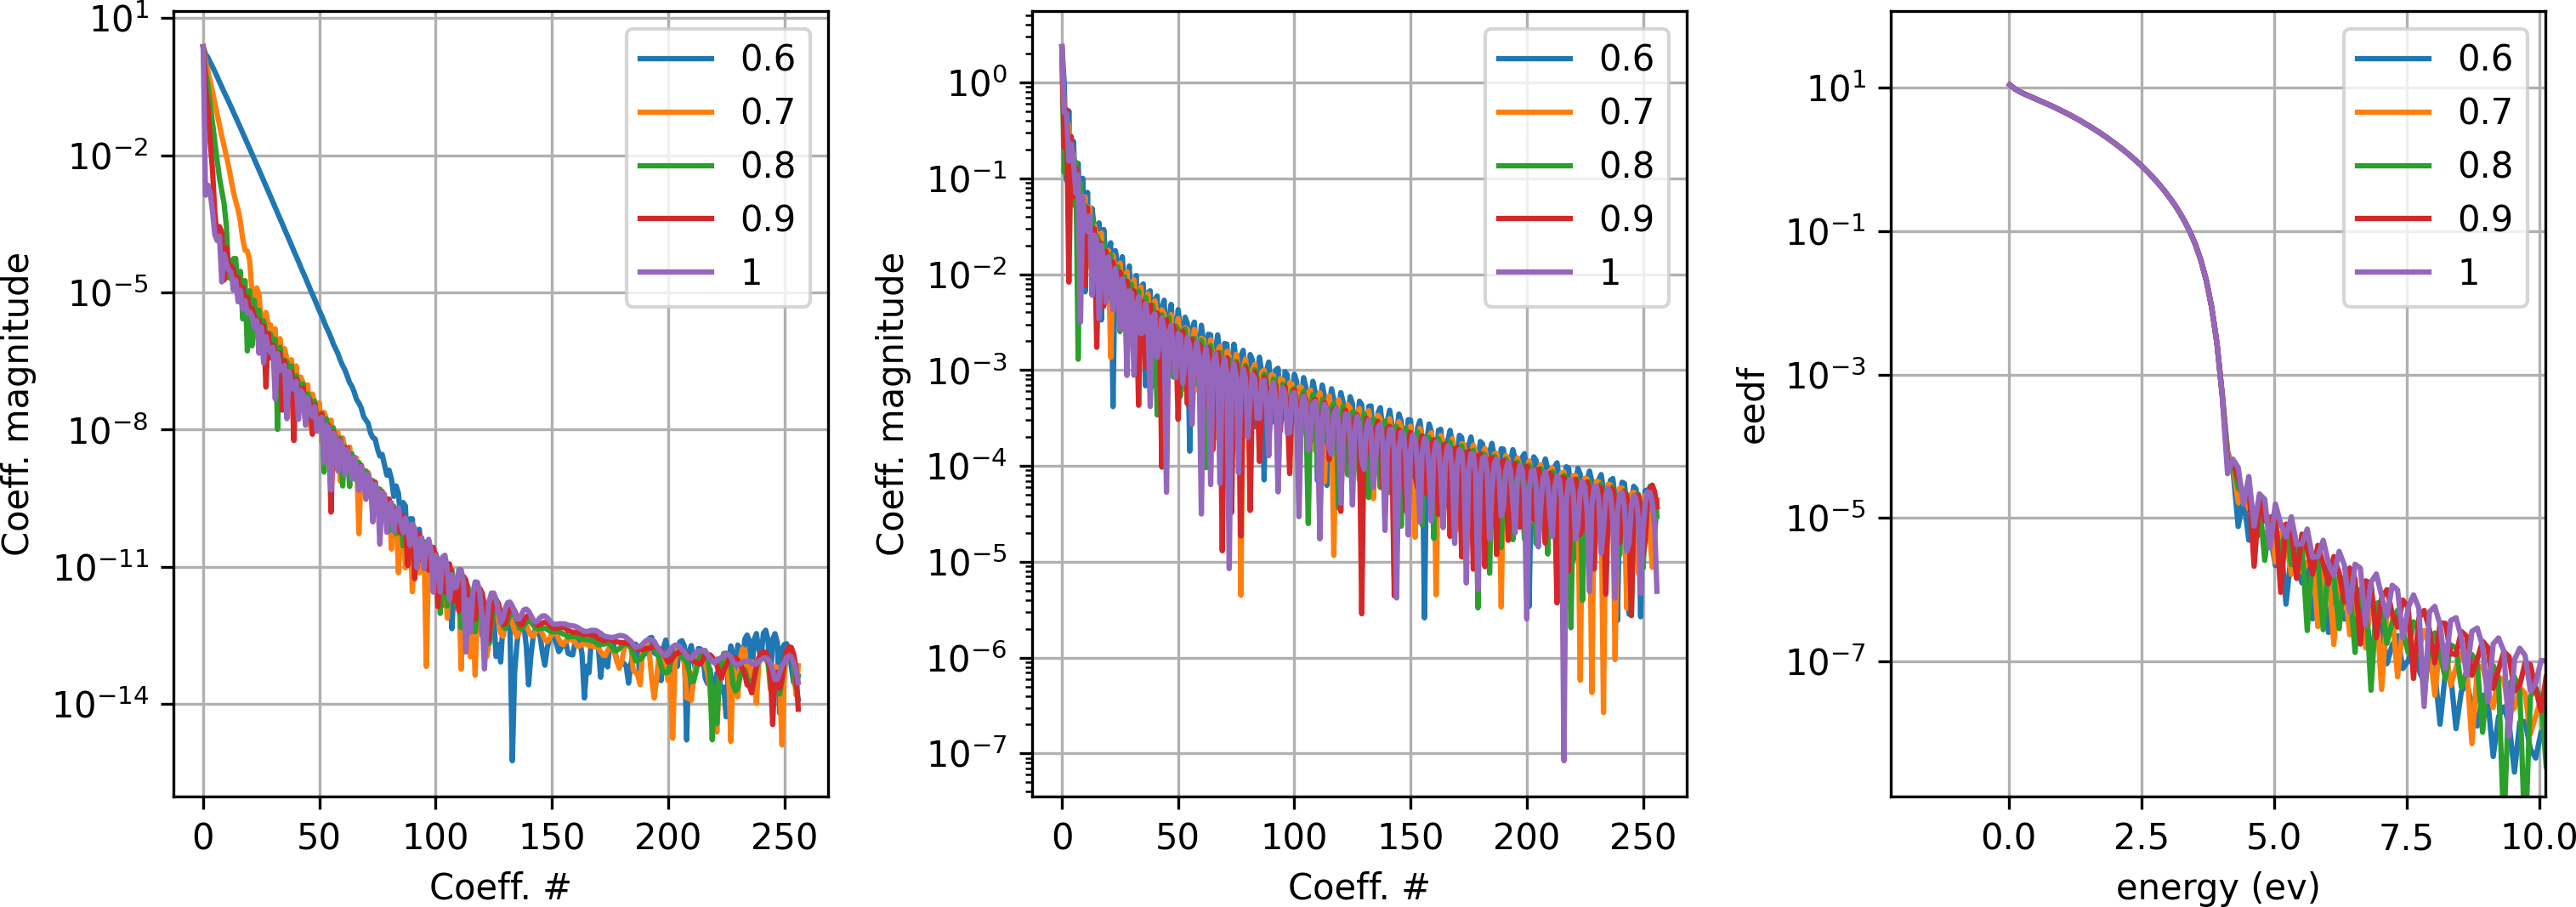
\includegraphics[width=0.99\textwidth]{fig/different_vth_real_1e-5.png}

%\begin{align*}
%\partial_t\of{a\of{t} f\of{t,\vect{v}}} + \vect{E} \cdot \nabla_\vect{v}\of{a\of{t} f\of{t,\vect{v}}}  & = C\of{a(t) f(t, \vect{v})} \\
%\dot{a}\of{t}f\of{t,\vect{v}} + a\of{t} \dot{f}\of{t,\vect{v}} +  a\of{t} \vect{E} \cdot \nabla_\vect{v}\of{f\of{t,\vect{v}}} &= C\of{a(t) f(t, \vect{v})}\\
%\end{align*}



%Attempt to compute the steady state solution analytically for B-splines. 
%\begin{align*}
%f\of{\vect{v},t} = \sum h_{klm}\of{t} \Phi_{kl}\of{\vr} Y_{lm}\of{\vtheta, \vphi}
%\end{align*}
%Total number of electrons
%\begin{align*}
%n = \myint_{R^3} f\of{\vect{v},t} d\vect{v} = \sum_{k} h_{k00}\of{t} \myint_{R^3} \Phi_{k0}\of{\vr} Y_{00}\of{\vtheta, \vphi} d\vect{v} = W_{p00}^T h_{p00}
%\end{align*} where $W_{p00} = \myint_{R^3} \Phi_{k0}\of{\vr} Y_{00}\of{\vtheta, \vphi} d\vect{v} $.
%
%\begin{align*}
%\vect{h} = 
%\begin{pmatrix}
%h_{k00} \\ \vect{h}_\ast
%\end{pmatrix}
%,\quad
%E = 
%\begin{pmatrix}
%0 & \vect{0}^T \\
%\vect{e}_{0\ast} & E_{\ast\ast}
%\end{pmatrix}
%,\quad
%C = 
%\begin{pmatrix}
%C_{00} & \vect{c}_{\ast 0}^T \\
%\vect{c}_{0\ast} & C_{\ast\ast}
%\end{pmatrix}
%\end{align*}


%
%\newpage
%
%\begin{align*}
%\vect{h} =
%\begin{pmatrix}
%h_0 \\
%\tilde{\vect{h}}
%\end{pmatrix}
%,\quad
%C = 
%\begin{pmatrix}
%0 & \vect{0}^T \\
%\vect{c}_0 & \tilde{C}
%\end{pmatrix}
%\end{align*}
%\begin{align*}
%\frac{d \tilde{\vect{h}}}{dt} = \tilde{C} \tilde{\vect{h}} + h_0 \vect{c}_0
%\end{align*}
%
%\begin{align*}
%\tilde{C} &= V \Lambda V^{-1}
%\end{align*}
%
%\begin{align*}
%\tilde{\vect{h}}\of{t} = V \exp\of{\Lambda t} V^{-1} \tilde{\vect{h}}\of{0} + h_0 V \left( I - \exp\of{\Lambda t} \right) \Lambda^{-1} V^{-1} \vect{c}_0
%\end{align*}
%
%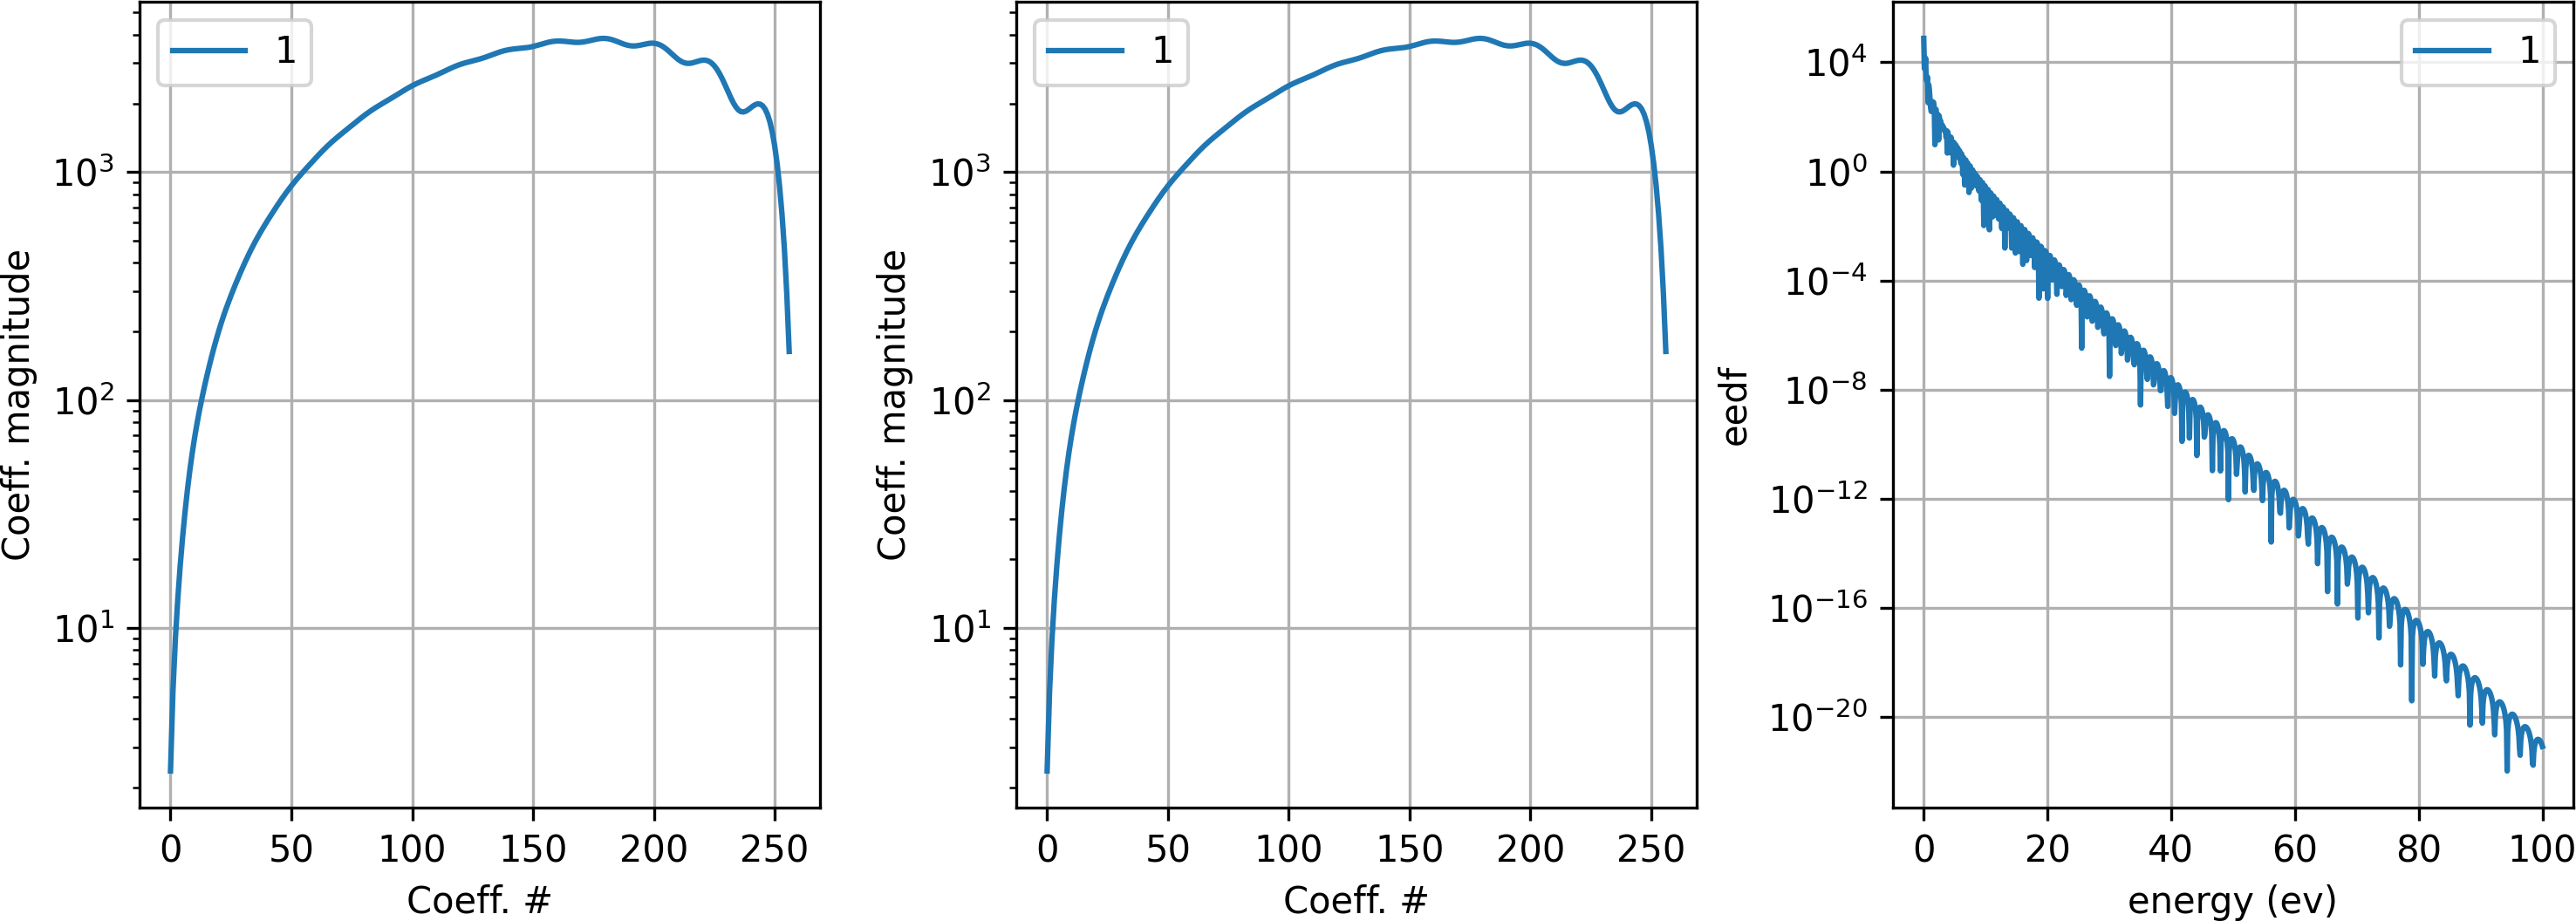
\includegraphics[width=0.99\textwidth]{fig/steady_state_elastic_only.png}
%
%\newpage
%System of ODEs for coefficients
%\begin{align*}
%\frac{d \vect{h}}{dt} - E \sin\of{\omega t} \vect{h} = C \vect{h}
%\end{align*}
%Eigenvalue decomposition of $C$:
%\begin{align*}
%C &= V \Lambda V^{-1}
%\end{align*}
%Change of variables:
%\begin{align*}
%\vect{y} &= V^{-1} \vect{h} \\
%F &= V^{-1} E V
%\end{align*}
%New form:
%\begin{align*}
%\frac{d \vect{y}}{dt} - F \sin\of{\omega t} \vect{y} = \Lambda \vect{y}
%\end{align*}
%A Floquet-Lyapunov transformation:
%\begin{align*}
%\vect{y} = \exp\of{-\frac{F}{\omega} \cos{\omega t} + \Lambda t} \vect{z}
%\end{align*}
%leads to:
%\begin{align*}
%\frac{d \vect{z}}{dt} = 0
%\end{align*}
%thus:
%\begin{align*}
%\vect{h}\of{t} = V \exp\of{\frac{V^{-1} E V}{\omega}  \left(1 - \cos\of{\omega t} \right) + \Lambda t} V^{-1} \vect{h}\of{0}
%\end{align*}
%
%\newpage
%\begin{align*}
%\vect{h} =
%\begin{pmatrix}
%h_0 \\
%\tilde{\vect{h}}
%\end{pmatrix}
%,\quad
%C = 
%\begin{pmatrix}
%0 & \vect{0}^T \\
%\vect{c}_0 & \tilde{C}
%\end{pmatrix}
%\end{align*}
%\begin{align*}
%\frac{d \tilde{\vect{h}}}{dt} - E \sin\of{\omega t} \tilde{\vect{h}} = \tilde{C} \tilde{\vect{h}} + h_0 \vect{c}_0
%\end{align*}
%Change of variables:
%\begin{align*}
%\vect{y} &= \tilde{V}^{-1} \tilde{\vect{h}} \\
%F &= \tilde{V}^{-1} \tilde{E} \tilde{V}\\
%\vect{g} &= \tilde{V}^{-1} h_0 \vect{c}_0
%\end{align*}
%New form:
%\begin{align*}
%\frac{d \vect{y}}{dt} - F \sin\of{\omega t} \vect{y} = \Lambda \vect{y} + \vect{g}
%\end{align*}
%After a Floquet-Lyapunov transformation:
%\begin{align*}
%\exp\of{-\frac{F}{\omega} \cos{\omega t} + \Lambda t} \frac{d \vect{z}}{dt} = \vect{g}
%\end{align*}
%Solving:
%\begin{align*}
%\vect{z}\of{t} = \vect{z}\of{0} + \int_{0}^{t} \exp\of{\frac{F}{\omega} \cos{\omega \tau} - \Lambda \tau} d\tau \vect{g} 
%\end{align*}
%
%\begin{multline*}
%\tilde{\vect{h}}\of{t} = \tilde{V} \exp\of{\frac{\tilde{V}^{-1} \tilde{E} \tilde{V}}{\omega} \left(1 - \cos\of{\omega t}\right) + \Lambda t} V^{-1} \tilde{\vect{h}}\of{0}
%\\
%+
%h_0
%\tilde{V} 
%\int_{0}^{t} \exp\of{\frac{\tilde{V}^{-1} \tilde{E} \tilde{V}}{\omega} \left( \cos\of{\omega \tau} - \cos\of{\omega t} \right)  - \Lambda \left( \tau - t \right)} d\tau V^{-1} \vect{c}_0
%\end{multline*}
